% ============================================================
% 第13章：函数在无穷远处的极限——水平渐近线
% ============================================================

\chapter{函数在无穷远处的极限——水平渐近线}

\begin{applicationbox}
\textbf{学完本章你能做什么？}
\begin{enumerate}
  \item 理解函数在 \(x \to \infty\) 时的极限——数列极限的自然延伸
  \item 区分\textbf{水平渐近线}（有极限）和\textbf{无穷极限}（无界）
  \item 对比不同函数的增长速度：\(\ln x, \sqrt{x}, x, x^2, e^x\)
\end{enumerate}
\end{applicationbox}


% ============================================================
\section{从数列到函数——从离散到连续}
% ============================================================

数列极限讲的是当 \(n \to \infty\)（正整数趋向无穷）时 \(a_n\) 的行为。

函数极限讲的是当 \(x \to \infty\)（实数趋向无穷）时 \(f(x)\) 的行为。

\begin{center}
\begin{tabular}{c|c}
\textbf{数列} & \textbf{函数} \\
\hline
\(n\) 只能取正整数 & \(x\) 可取任意实数 \\
\(\displaystyle\lim_{n\to\infty} a_n = L\) & \(\displaystyle\lim_{x\to\infty} f(x) = L\) \\
离散的点 & 连续的曲线 \\
\end{tabular}
\end{center}


% ============================================================
\section{\(x \to \infty\) 时的极限}
% ============================================================

\begin{definitionbox}[函数在无穷远处的极限]
如果当 \(x\) 越来越大时，\(f(x)\) 无限趋近于一个固定的数 \(L\)，
则称 \(L\) 是函数 \(f\) 当 \(x \to \infty\) 时的\textbf{极限}。

记作 \(\displaystyle \lim_{x \to \infty} f(x) = L\)。

\textbf{ε-N 定义：} 对任意 \(\varepsilon>0\)，存在 \(X>0\)，使得当 \(x>X\) 时，
\[
|f(x)-L| < \varepsilon
\]
当 \(x \to -\infty\) 时类似：存在 \(X<0\) 使 \(x<X\) 时 \(|f(x)-L|<\varepsilon\)。
\end{definitionbox}

\begin{examplebox}[1——水平渐近线]
\begin{center}
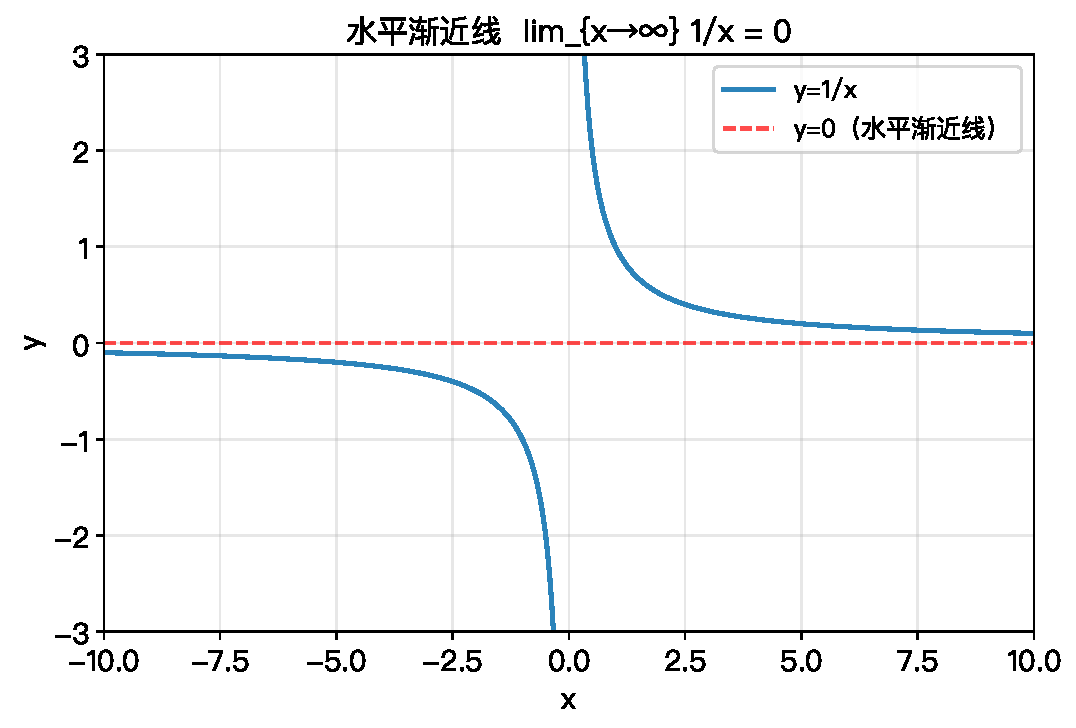
\includegraphics[width=0.7\textwidth]{figures/ch13_horizontal_asymptote.pdf}
\end{center}

\[
\lim_{x \to \infty} \frac{1}{x} = 0,\qquad
\lim_{x \to -\infty} \frac{1}{x} = 0
\]

\textbf{几何意义：} 直线 \(y = 0\) 是函数的\textbf{水平渐近线}。
当 \(x\) 趋向无穷时，曲线无限接近这条线，但永远不碰到（\(x\) 有限时）。
\end{examplebox}


% ============================================================
\section{不同函数的增长速度}
% ============================================================

\begin{examplebox}[2——增长速度的"等级"]
\begin{center}
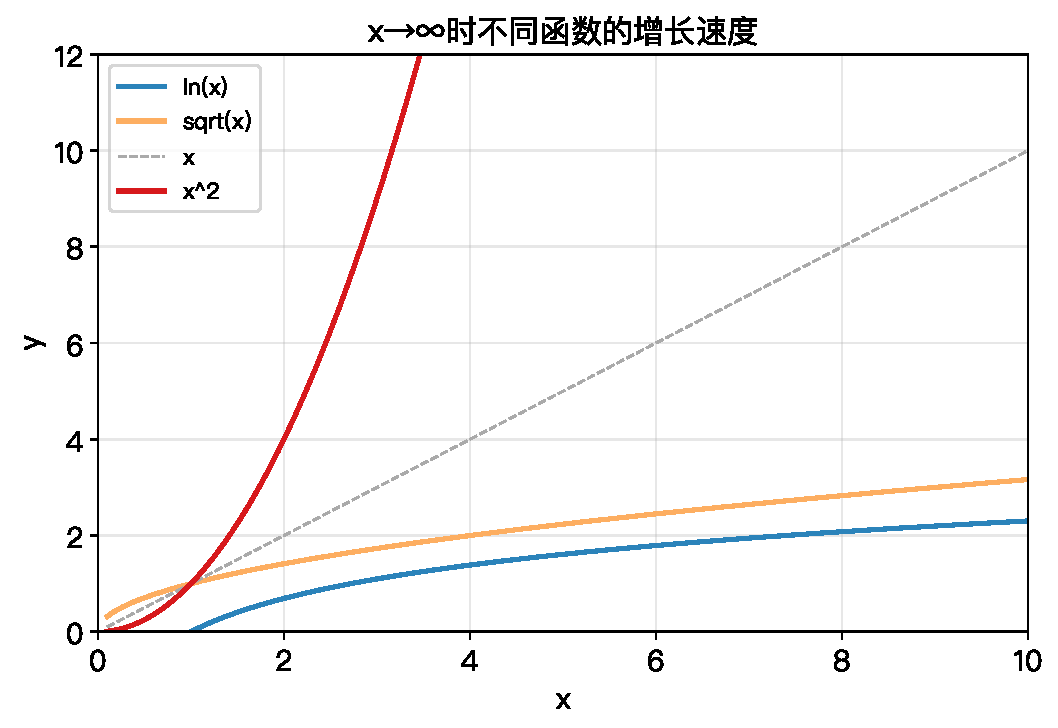
\includegraphics[width=0.7\textwidth]{figures/ch13_growth_rates.pdf}
\end{center}

当 \(x \to \infty\) 时，增长速度从慢到快：
\[
\ln x \;\ll\; \sqrt{x} \;\ll\; x \;\ll\; x^2 \;\ll\; x^3 \;\ll\; e^x \;\ll\; 2^x
\]

\textbf{重要结论：}
\begin{itemize}
  \item 对数增长最慢（\(\ln x\)）
  \item 幂函数 \(x^k\) 按指数 \(k\) 分等级
  \item 指数函数 \(e^x\) 碾压所有幂函数
\end{itemize}
\end{examplebox}


% ============================================================
\section{\(x \to a\) 时的无穷极限}
% ============================================================

\begin{definitionbox}[无穷极限]
如果当 \(x\) 趋近于 \(a\) 时，\(f(x)\) 的绝对值无限增大，
则称 \(f(x)\) 在 \(x=a\) 处\textbf{趋于无穷}。

记作 \(\displaystyle \lim_{x \to a} f(x) = \infty\)（或 \(-\infty\)），此时 \(x=a\) 是\textbf{垂直渐近线}。

\textbf{ε-δ 定义：} 对任意 \(M>0\)，存在 \(\delta>0\)，使得当 \(0<|x-a|<\delta\) 时，
\(f(x) > M\)（或 \(f(x) < -M\)）。
\end{definitionbox}

\begin{examplebox}[3——垂直渐近线]
\begin{center}
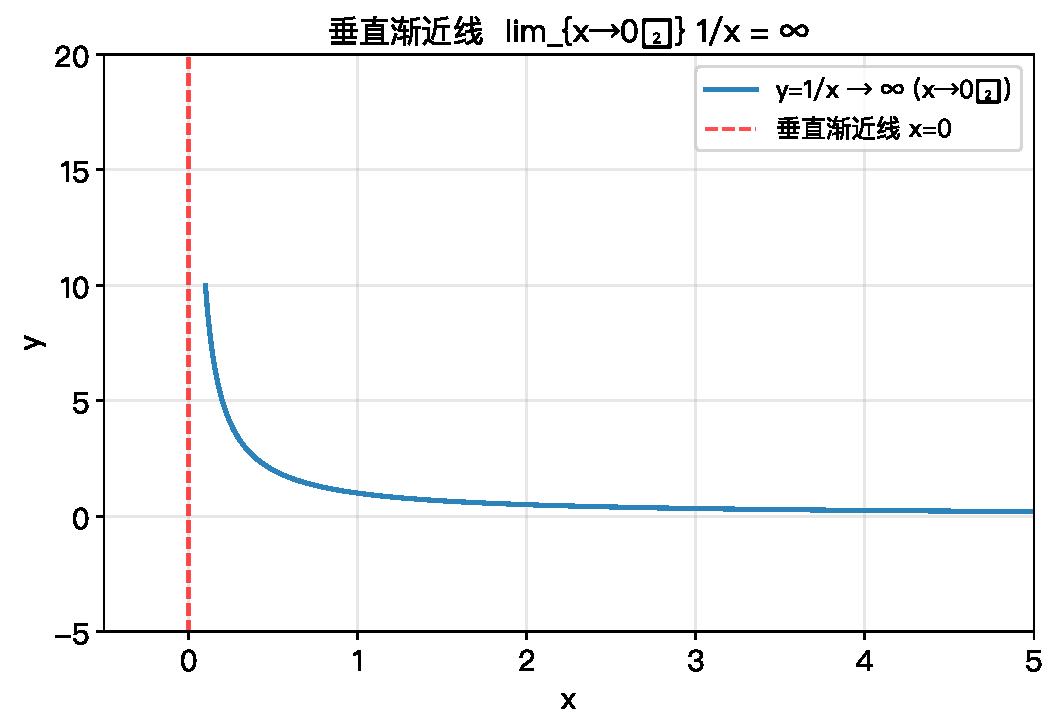
\includegraphics[width=0.7\textwidth]{figures/ch13_vertical_asymptote.pdf}
\end{center}

\[
\lim_{x \to 0^+} \frac{1}{x} = +\infty,\qquad
\lim_{x \to 0^-} \frac{1}{x} = -\infty
\]

\(x = 0\) 是 \(y = 1/x\) 的\textbf{垂直渐近线}。
当 \(x\) 从右侧趋近 0 时，函数值趋向正无穷；
从左侧趋近 0 时，函数值趋向负无穷。
\end{examplebox}


% ============================================================
\section{本章小结}
% ============================================================

\begin{progressbox}
\textbf{函数在无穷远处的极限}：\(\lim_{x \to \infty} f(x) = L\) 对应水平渐近线 \(y = L\)

\textbf{无穷极限}：\(\lim_{x \to a} f(x) = \infty\) 对应垂直渐近线 \(x = a\)

\textbf{增长速度等级}：\(\ln x < \sqrt{x} < x < x^2 < x^3 < e^x\)
\end{progressbox}


% ============================================================
% 习题
% ============================================================
\section{习题}

\begin{exercise}[0]
求 \(\displaystyle\lim_{x\to\infty} \frac{1}{x}\)。
\end{exercise}
\begin{exercise}[0]
函数 \(y=1/x\) 的水平渐近线是什么？
\end{exercise}
\begin{exercise}[0]
函数 \(y=1/x\) 的垂直渐近线是什么？
\end{exercise}
\begin{exercise}[0]
判断：\(\displaystyle\lim_{x\to\infty} e^x\) 是有限数吗？
\end{exercise}

\begin{exercise}[1]
求 \(\displaystyle\lim_{x\to\infty} \frac{2}{x+1}\)。
\end{exercise}
\begin{exercise}[1]
求 \(\displaystyle\lim_{x\to-\infty} \frac{1}{x^2}\)。
\end{exercise}
\begin{exercise}[1]
比较大小（\(x\) 很大时）：\(x^{100}\) 和 \(1.001^x\) 哪个增长更快？
\end{exercise}
\begin{exercise}[1]
判断：若 \(\lim_{x\to\infty} f(x)=5\)，则 \(y=5\) 是一条什么线？
\end{exercise}

\begin{exercise}[2]
求 \(\displaystyle\lim_{x\to\infty} \frac{2x+1}{x-3}\)。
\end{exercise}
\begin{exercise}[2]
求 \(\displaystyle\lim_{x\to\infty} \frac{x^2+1}{3x^2-2x}\)。
\end{exercise}
\begin{exercise}[2]
求 \(\displaystyle\lim_{x\to 0^+} \ln x\)（提示：\(\ln x \to -\infty\)）。
\end{exercise}
\begin{exercise}[2]
函数 \(y=\frac{1}{(x-2)^2}\) 的垂直渐近线在哪里？
\end{exercise}

\begin{exercise}[3]
求 \(\displaystyle\lim_{x\to\infty} (\sqrt{x+1}-\sqrt{x})\)。
\end{exercise}
\begin{exercise}[3]
求水平渐近线：\(y=\frac{2x^2+1}{x^2-4}\)。
\end{exercise}
\begin{exercise}[3]
求垂直渐近线：\(y=\frac{x}{x^2-1}\)。
\end{exercise}
\begin{exercise}[3]
比较 \(\lim_{x\to\infty} \frac{x^{10}}{2^x}\) 和 \(\lim_{x\to\infty} \frac{2^x}{x^{10}}\)。
\end{exercise}
\begin{exercise}[3]
某药的血药浓度 \(C(t)=\frac{100t}{t+2}\)，求 \(t\to\infty\) 时的极限浓度。
\end{exercise}

\begin{exercise}[4]
求 \(\displaystyle\lim_{x\to\infty} \left(\frac{x+1}{x-1}\right)^x\)。
\end{exercise}
\begin{exercise}[4]
证明 \(\displaystyle\lim_{x\to\infty} \frac{\ln x}{x} = 0\)。
\end{exercise}
\begin{exercise}[4]
求渐近线：\(y=\frac{x^2+1}{x}\)（提示：有斜渐近线）。
\end{exercise}
\begin{exercise}[4]
函数 \(f(x)=\frac{e^x}{e^x+1}\)，求水平渐近线。
\end{exercise}
\begin{exercise}[4]
求 \(\displaystyle\lim_{x\to\infty} \frac{\sin x}{x}\)。
\end{exercise}

\begin{exercise}[5]
证明 \(\displaystyle\lim_{x\to\infty} \frac{x^k}{e^x}=0\) 对任意正整数 \(k\) 成立。
\end{exercise}
\begin{exercise}[5]
求 \(\displaystyle\lim_{x\to 0} \frac{1}{x^2}\) 并从左右两侧讨论。
\end{exercise}
\begin{exercise}[5]
函数 \(y=\frac{2x^2+3x+1}{x^2-5x+6}\) 的水平和垂直渐近线。
\end{exercise}
\begin{exercise}[5]
求 \(\displaystyle\lim_{x\to\infty} x\sin\frac{1}{x}\)。
\end{exercise}

\begin{exercise}[6]
证明 \(\displaystyle\lim_{x\to\infty} \left(1+\frac{1}{x}\right)^x = e\)。
\end{exercise}
\begin{exercise}[6]
求 \(\displaystyle\lim_{x\to 0^+} x\ln x\)。
\end{exercise}
\begin{exercise}[6]
求 \(\displaystyle\lim_{x\to\infty} \frac{\ln(1+e^x)}{x}\)。
\end{exercise}

\begin{exercise}[7]
设 \(f(x)=\frac{x^n}{e^x}\)（\(n\) 为正整数）。
\begin{enumerate}
  \item[(1)] 证明存在 \(X\) 使 \(x>X\) 时 \(f(x)<\frac{1}{x}\)
  \item[(2)] 求 \(\lim_{x\to\infty} f(x)\)
\end{enumerate}
\end{exercise}

